% est�mme ihme "underfull \hbox (badness 10000)" -varoitukset (ei hajua mist� tulevat)
\hbadness=10000


\section{Introduction}

This document tells how the student project at the Department of Computer Science of University of Helsinki for building a new user interface for the SQUID magnetometer at the Department of Geophysics of the University of Helsinki went. The clients were Lauri Pesonen with his assistants Fabio Donadini and Tomas Kohout from the Department of Geophysics.

The name of the produced program is Ikayaki. The name comes from a japanese seafood - dried, grilled squid.

The project took place from 25.1.2005 to 6.5.2005.


\section{Organization}

The people related to this project are shown in Figure~\ref{fig:organization}.

\begin{figure}[h]
\begin{tabular}{lll}
{\bf Name} & {\bf Role} & {\bf E-Mail} \\
\hline
Mikko Jormalainen	& Project Team			& mtjormal@cc.helsinki.fi \\
Samuli Kaipiainen	& Project Team			& samuli.kaipiainen@cs.helsinki.fi \\
Aki Korpua		& Project Team			& aki.korpua@cs.helsinki.fi \\
Esko Luontola		& Project Team (Manager)	& esko.luontola@cs.helsinki.fi \\
Aki Sysm�l�inen		& Project Team			& aki.sysmalainen@helsinki.fi \\
\hline
Lauri J. Pesonen	& Client			& lauri.pesonen@helsinki.fi \\
Tomas Kohout		& Client			& tomas.kohout@helsinki.fi \\
Fabio Donadini		& Client			& fabio.donadini@helsinki.fi \\
\hline
Juha Taina		& Course Manager		& taina@cs.helsinki.fi \\
Jenni Valorinta		& Instructor			& valorint@cs.helsinki.fi
\end{tabular}
\caption{The people who were part of this project}
\label{fig:organization}
\end{figure}


\section{Amount of Work}

The amount of work that the team did is shown in Figure~\ref{fig:workhours}.

\begin{figure}
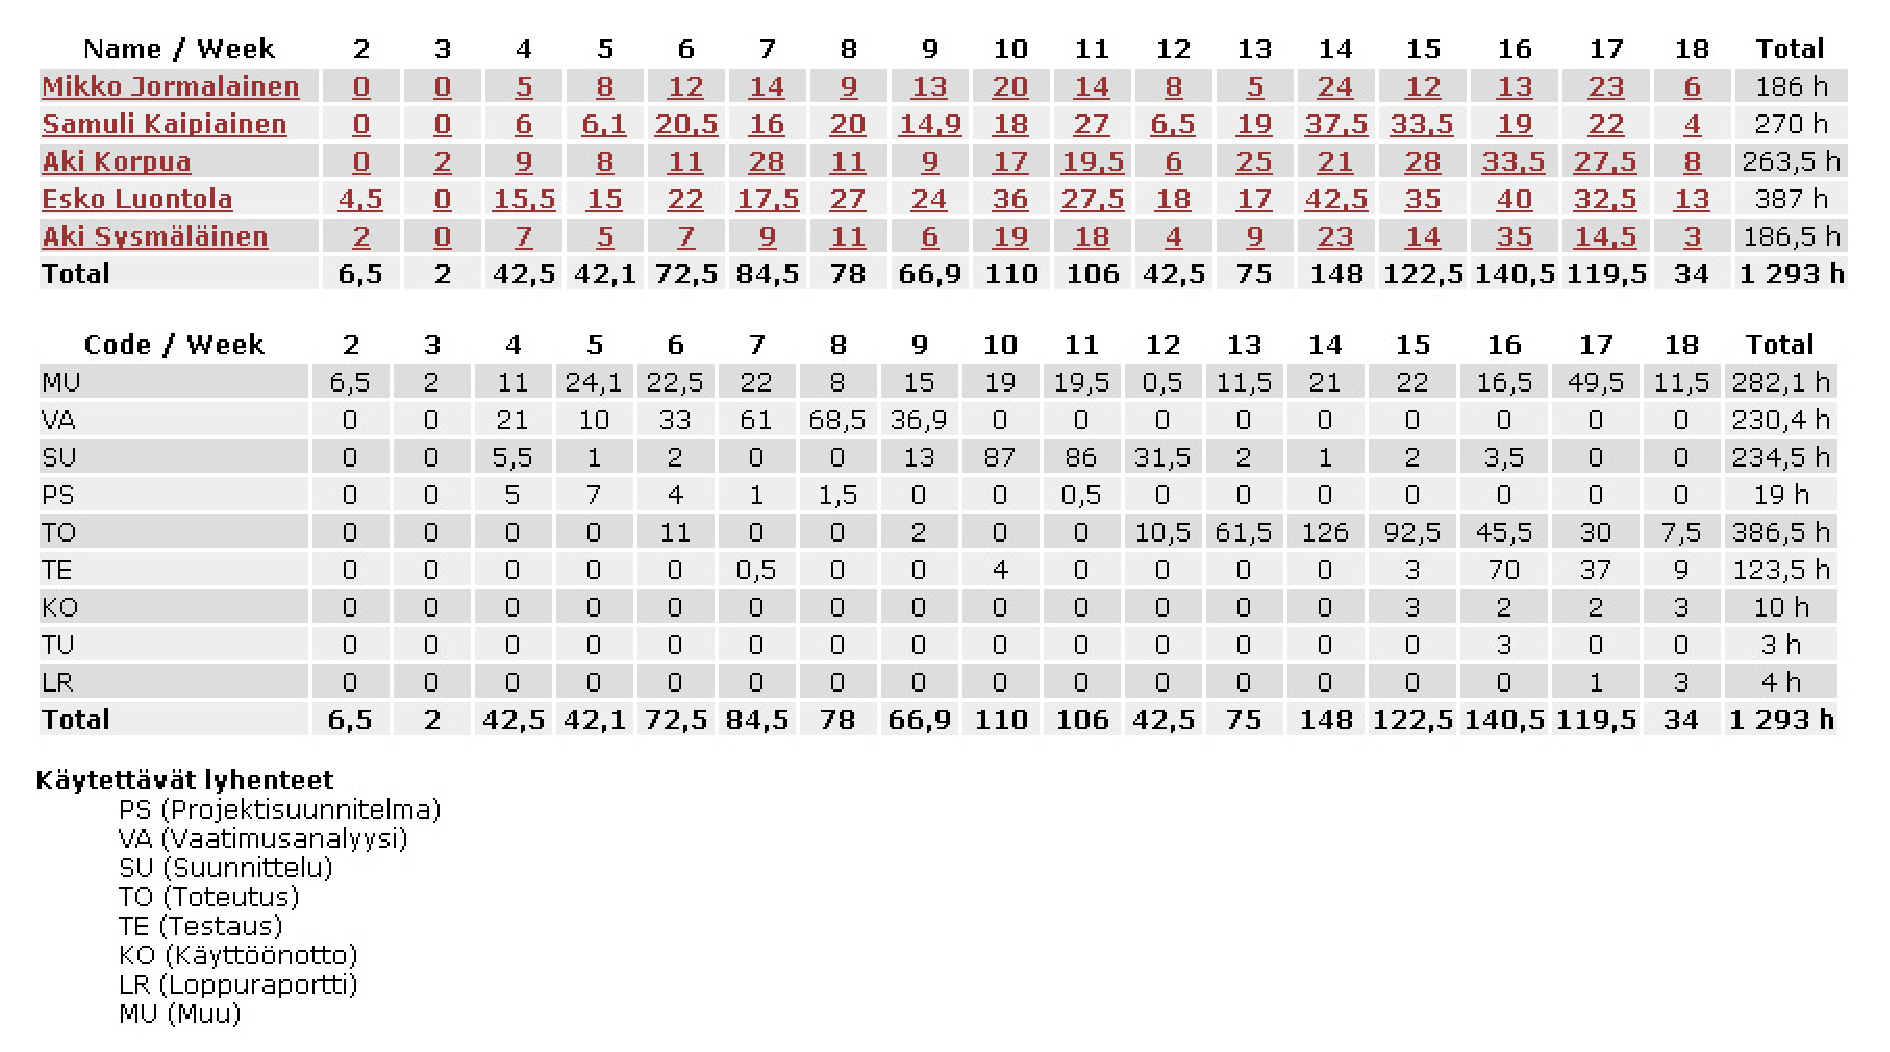
\includegraphics[width=22cm,angle=90]{workhours.eps}
\caption{How many hours of work the team members did.}
\label{fig:workhours}
\end{figure}

The estimated size of the program was a maximum of 13000 lines of code. The final size of the program is some 21500 lines of code. So the estimation that was made at the very beginning of the project (before the team even understood what they were doing ;) was more than 65\% too low.

During the project was also produced HourParser, a program for managing the team's work hours. Its size is 1000 lines of code.

The final schedule for the project is in Figure~\ref{fig:schedule}.


\begin{figure}[h]
\begin{tabular}{llll}
{\bf Task} & {\bf Start} & {\bf End} & {\bf Days} \\
\hline
Project Plan		& 25.1.2005	& 8.2.2005	& 14 \\
HourParser		& 8.2.2005	& 9.2.2005	& 1 \\
Definition		& 25.1.2005	& 1.3.2005	& 35 \\
- Prototype		&		& 24.2.2005	& \\
- Requirements Document	&		& 2.3.2005	& \\
Design			& 1.3.2005	& 22.3.2005	& 21  \\
- Design Document	&		& 22.3.2005	& \\
Production		& 22.3.2005	& 14.4.2005	& 23 \\
Testing			& 14.4.2005	& 28.4.2005	& 14 \\
- Testing Plan		&		& 22.4.2005	& \\
- Testing Report	&		& 29.4.2005	& \\
Installing		& 28.4.2005	& 5.5.2005	& 7 \\
- Final Report		&		& 3.5.2005	& \\
- User Manual		&		& xx.5.2005	& \\
- Realization Document	&		& xx.5.2005	& \\
\end{tabular}
\caption{Final project schedule}
\label{fig:schedule}
\end{figure}


\section{Debriefing}

The writings in this section are based on the answers that the project team members gave to a bunch of questions.

% \begin{itemize}
% \item How did you like the theme of the program?
% \item How was the project in general?
% \item How has the project team been?
% \item How was the amount of work?
% \item What did you learn?
% \end{itemize}
% 
% \begin{itemize}
% \item Where have we succeeded and where failed?
% \item What should have been done better?
% \item What do you think about the tools and techniques that were used? Which of them would your recommend to others? (goal-derived UI design, meetings, hour management, email, irc, Java, Swing, Latex, Dia, CVS, IntelliJ IDEA, JGoodies Looks, virtual serial ports, JUnit, XML...)
% \item What do you think about the project model that was used? (waterfall model)
% \item How was the relation of the design and the production? Could something have been expected or done differently?
% \item How did the time table change from what was planned? Why were there changes and what effects did they have?
% \item What problems did the existing hardware, software and their documentation bring? How were the problems solved?
% \end{itemize}
% 
% \begin{itemize}
% \item Describe shortly the operation of the client.
% \item How was it to work with an English speaking client? How did it affect the project?
% \item How did the instructor do her work?
% \item Evaluate the operation of each team member, also yourself. If you would describe each one of them with one word, what would that be?
% \end{itemize}


\subsection{Overview}

The project has been a lot of work, some pain, some nice moments and reasonable enough results. Everybody in the team though that the theme of the program was both challenging and interesting. It was motivating to solve some real-world problems, even when it was out of our world. Nobody from the development team knew anything about the subject when the project got started started, and it took some weeks to understand what the people at Geophysics are actually doing and what it was that they really wanted. At start everything as a bit confusing and stressful, but towards the end the project team got more and more confident about the result.

The team was strong and people were supporting each other well. There were only five guys doing it all, and sicknesses and other courses took a huge amount of time from the project. The amount of work was much and it was shared unevenly. It took some time before the whole team was functional, but the team improved during the project and chemistry between the team members got better and better.

All team members learned working in a team. Some other things that were learned are: diplomatic negotiation skills with the client, the importance of meetings, the importance of design and that feeble feeling of things falling apart. Some technical things that were learned: Latex, CVS, more Java, new features of Java 1.5, IRC. The English of some students improved.


\subsection{Project}

The team has succeeded in making a program that works and the client appears to be pleased with it. The team mostly succeeded in everything, but failed to put the last effort and add a finishing touch to every step. The meetings with the client and communication could have been better, and as a result it was not possible to guess all of the requirements that the client would have wanted. The user requirements and the program could have been designed better. Testing the program was not as thorough as it should have been. The work did not keep up with the schedule, so in the end there was more work than in the beginning. The work load could have been distributed better.

What the project team thinks about the following:

\begin{itemize}
\item Goal-Derived UI Design: \\
	The UI would never have been even nearly as good if we would not have payed special attention to it. User observations gave us a better idea about client's workflow with the old software. The prototypes were also essential in designing the program.
\item Meetings: \\
	Needed for the people to communicate. Things could work in plain irc/email, but not when everyone is committed enough to it, so regular meetings are needed.
\item Hour management with HourParser: \\
	Great system, it's good that other members can see your hours right a way. The created program is much better than any previous ones. :) Other teams should try it.
\item E-Mail: \\
	Good for coordination and communication. Mailing lists are good for communication within the project team. Much of the communication with the client was by e-mail.
\item IRC: \\
	Was in important role when we were not working face-to-face, which was the case in about 90\% of all work. Has been very helpful when many people are working on the same thing at the same time, especially so right before a deadline. It was also possible that while some are testing with the SQUID equipment, others stay home and program fixes for the found bugs, so that they can be tested right away.
\item Java and Swing: \\
	Good choice here. It's a safe choice when the coders are not too experienced. It would never have been possible for all to learn C++ well enough to make a program half this complicated. Performance was not a program with current hardware.
\item Latex: \\
	Hell and pain. Chainsaw internals massacre.
\item Dia: \\
	At least the Windows version was buggy and the UI was designed to kill. Missed code generating features. A better tool for writing UML would be needed.
\item CVS: \\
	Necessary for file management, even if a bit limited (can not rename/move files). The commandline version is clumsy - keep away from it. IDEA has a nice CVS front-end and propably so have many other IDEs.
\item IntelliJ IDEA: \\
	Really well designed IDE for Java coding. The UI Designer makes the creation of complex layouts easy. For example it took for a first-timer only about 30 minutes to make the device configuration dialog's layout. Only stupid people write Java GUIs 100\% by hand. :P
\item JGoodies Looks: \\
	Looks better than the standard Swing look.
\item Virtual serial ports: \\
	Helped at some point a lot. Was a necessity for the development of serial API.
\item JUnit: \\
	Could have been used more. The team did not get too much in to it, but it worked well for serial testing.
\item XML: \\
	Easy, effective and expandable. Was the best option for the new file format.
\end{itemize}

The waterfall project model that was used is a bit stiff, but it works. It is suitable for such short student projects as this. There would not have been time to use a more complicated model. The amount of documentation is a bit too much, though. A more flexible project model would be recommendable.

Those parts that were designed well, were produced according to the design. Those that were not designed, were produced more or less without plans. The user interface was produced accurately according to plans (use cases and prototypes) and so were also the Project data classes (ikayaki.*). The amount of time spent on designing could have been huge, but with this timetable the results were fair. If there had been time, the program requirements could have been more detailed (requires more communication with the client) and the program code could have been designed better (can be hard with GUI classes and their huge API).

Almost every phase was delayed, as expected. Maybe it would have hold better if the amount of work done by everyone were constant (20~h/week) all the time. Always someone (sometimes many) didn't do their jobs when supposed to; nothing much to help it, as everyone had other things than this project to do. Morale was low at times, which is inevitable in such a long project. The client also gave some extra requirements, which required some time to produce (luckily not too much). As a result, there was not enough time to test the program properly.

The legacy C code was a nightmare. If the team had known about the existense of protocol documentation, the old code could have been dumped sooner, because it was pretty hard to read and had no documentation. It was a good choice to start everything from ground. Using the old code would have created too many new risks and slowed down the project.

The protocol documentation was incomplete and did not mach the reality, so creating an emulator was not very useful. The created SerialProxy class gave much undocumented information about the protocol, so looking at how the old program does the things on protocol level made the day. Hardware was actually good and safe to use when you learned it, which helped a lot when testing and cleared errors in the documentation.


\subsection{People}

The client has been very interested in the project, which is good. There should have been more communication with the client, so that the team could have explained better things such as the process of software development. In the beginning the information from the client was sometimes inconsistent and the team did not always known who to follow, but this improved towards the end. The client was committed to project and ready to offer their help and time as much as they could. Special thanks to Fabio for being of much help.

Apparently most of the team members (4 out of 5) had never been talking that much English. The use of English slowed down the process in the beginning, but later on it was just a minor issue. Sometimes it was a bit hard to understand everything and sometimes it took time to find the right words, but it did not affect the project in the end. In overall the use of English has been good practice for the future.

The instructor did her work well, silently observing the project team when everything was going well and stepping in to direct when time was running out or the team was going to make a mistake. At very beginning there was some confusion about the authority between her and the project manager, but that was then sorted out. She kept the project and the group on trail and emphasized things that got less attention. She could have been a bit more relaxed on some issues when the internal pressure of the group was already high. But on the other side the pressure tolerances of the team got much better and more ready for real world challenges. In general she was nice and fair.


\subsubsection{Team members' evaluations of themselves}

\textbf{Mikko Jormalainen} \\
- Poor.

\textbf{Samuli Kaipiainen} \\
- Tried to do my jobs on time, some (but not many) failings to do so though, tried a couple of times to silently keep the project in one piece, lost some (or at few times, a lot) morale in the end.

\textbf{Aki Korpua} \\
- Lazy parasite. I was really working hard, but WoW and and other intrests took too much time.

\textbf{Esko Luontola} \\
- Maybe I worked a bit too much, but the work does not disappear by itself. Running a project team was new for me and what made it more difficult, was that everybody in the team were strangers at the beginning of the project. I'll try to improve in delegating work to others in the future. I know that I'm overconscientious.

\textbf{Aki Sysm�l�inen} \\
- At the beginning my use of time for the project was minimal but towards the end it got better. I was eager to take the lead when it was quiet on that front. I at least tried to add some diplomacy to client-project group relations.


\subsubsection{Team members' evaluations of each others}

\textbf{Mikko Jormalainen} \\
- That one guy. Could have been more in contact with other members. Did his work well anyway. \\
- Didn't have that much interest in the project, or so it seemed at the beginning, but not so much towards the end. Was most always ready to have a meeting of some sort. Had some weird problems with cvs updating frequency x) \\
- Communication was lagging quite much. Does he even have 24/7 internet access at home? \\
- Did his part in documenting. Could have done more coding. He was also a bit distant from the group from time to time.

\textbf{Samuli Kaipiainen} \\
- Does excellent work when he is into it. \\
- Did what was assigned to him and did it well. \\
- Good. \\
- Did a great job with the project explorer which is an achievement of usability. But when he got full of the coding the whole group got a bit affected by that. His sense of humor and analytic attitude on problems were invaluable to group and the project.

\textbf{Aki Korpua} \\
- Fast worker, didn't care so much for perfection :) Did his part even when tired and out of morale. Had some good sympathy for the clients, which drove him to try and make a working final software. \\
- Was also good in what he did. Did a good job in digging into the SQUID and the old program. Had time for the project in spite of WoW. :) \\
- Good. \\
- He did a lot of work with interface and emulator. Some of his emotional reactions at the beginning distracted other group members. His support and hard work kept the group going during the black spots.

\textbf{Esko Luontola} \\
- Hero. Kept our project alive. Could have taken more leader role at the beginning. \\
- Kept the project in one piece. Did something like 80\% of all coding, and was good at it too. Didn't care (or so it seemed) about work hours being accumulated to him. Made some vague changes to others' codings =) \\
- Excellent. \\
- At the start it took some time of him to take the lead but after that he's work has been pretty convincing. His contribution to coding was huge and he kept the code together and fixed and added a lot to other guys coding.

\textbf{Aki Sysm�l�inen} \\
- Sleepyhead, hehe. Dont try to do all courses at same time. Good social skills and does his work good. \\
- Had many other project going on at the same time 8) But, did his part in the end, such as the graphs for the program, which would have been a shame not to have. Took the lead sometimes, when things didn't go forwards. \\
- Was a bit too busy with life outside the project. Was good in asking questions for example when designing the UI. Also good in communicating with the client. \\
- OK.


